% !TEX encoding = UTF-8 Unicode
\documentclass[a4paper]{article}

\usepackage{color}
\usepackage{url}
\usepackage[T2A]{fontenc} % enable Cyrillic fonts
\usepackage[utf8]{inputenc} % make weird characters work
\usepackage{graphicx}

\usepackage[english,serbian]{babel}
%\usepackage[english,serbianc]{babel} %ukljuciti babel sa ovim opcijama, umesto gornjim, ukoliko se koristi cirilica

\usepackage[unicode]{hyperref}
\hypersetup{colorlinks,citecolor=green,filecolor=green,linkcolor=blue,urlcolor=blue}

\usepackage{listings}

%\newtheorem{primer}{Пример}[section] %ćirilični primer
\newtheorem{primer}{Primer}[section]

\definecolor{mygreen}{rgb}{0,0.6,0}
\definecolor{mygray}{rgb}{0.5,0.5,0.5}
\definecolor{mymauve}{rgb}{0.58,0,0.82}

\lstset{ 
  backgroundcolor=\color{white},   % choose the background color; you must add \usepackage{color} or \usepackage{xcolor}; should come as last argument
  basicstyle=\scriptsize\ttfamily,        % the size of the fonts that are used for the code
  breakatwhitespace=false,         % sets if automatic breaks should only happen at whitespace
  breaklines=true,                 % sets automatic line breaking
  captionpos=b,                    % sets the caption-position to bottom
  commentstyle=\color{mygreen},    % comment style
  deletekeywords={...},            % if you want to delete keywords from the given language
  escapeinside={\%*}{*)},          % if you want to add LaTeX within your code
  extendedchars=true,              % lets you use non-ASCII characters; for 8-bits encodings only, does not work with UTF-8
  firstnumber=1000,                % start line enumeration with line 1000
  frame=single,	                   % adds a frame around the code
  keepspaces=true,                 % keeps spaces in text, useful for keeping indentation of code (possibly needs columns=flexible)
  keywordstyle=\color{blue},       % keyword style
  language=Python,                 % the language of the code
  morekeywords={*,...},            % if you want to add more keywords to the set
  numbers=left,                    % where to put the line-numbers; possible values are (none, left, right)
  numbersep=5pt,                   % how far the line-numbers are from the code
  numberstyle=\tiny\color{mygray}, % the style that is used for the line-numbers
  rulecolor=\color{black},         % if not set, the frame-color may be changed on line-breaks within not-black text (e.g. comments (green here))
  showspaces=false,                % show spaces everywhere adding particular underscores; it overrides 'showstringspaces'
  showstringspaces=false,          % underline spaces within strings only
  showtabs=false,                  % show tabs within strings adding particular underscores
  stepnumber=2,                    % the step between two line-numbers. If it's 1, each line will be numbered
  stringstyle=\color{mymauve},     % string literal style
  tabsize=2,	                   % sets default tabsize to 2 spaces
  title=\lstname                   % show the filename of files included with \lstinputlisting; also try caption instead of title
}

\begin{document}

\section{Autonomna vozila}
\label{sec:Autonomna vozila}
Automobilska industija je još jedna delatnost u kojoj je vestačka inteligencija sve više zastupljena. Autonomna vozila kao takva su veoma interesantna i kompleksna tema, kako iz aspekta nauke i samog njihovog razvoja, tako i iz aspekta etike. \\
Naime, izvršena je podela ovih vozila prema stepenu automatizacije:
\begin{itemize}
 \item {Stepen 1 - Jedini stepen automatizacije koji poseduje vozilo je sistem za           držanje rastojanja.}
 \item {Stepen 2 - Vozilo poseduje sisteme za praćenje pravca i samostalno                  parkiranje.}
 \item {Stepen 3 - Vozilo poseduje sistem za autonomnu vožnju, ali ukoliko dođe do          nekih poteškoća poput vremenskih nepogoda, signalizira čoveku da treba da         preuzme kontrolu.}
 \item {Stepen 4 - Vozilo poseduje sistem za autonomnu vožnju, ali u slučaju nekih              problema na putu, vozilo će se samo bezbedno zaustaviti, bez zahtevanja da        čovek preuzme kontrolu.}
 \item {Stepen 5 - Potpuna automatizacija vožnje i prevazilaženje prepreka.}
\end{itemize} 
Poslednih godina kompanije sve više novca ulažu u razvoj ovih vozila, a vodeće države po broju patenata se mogu videti na slici \ref{fig:histograma}.

\begin{figure}[h!]
\begin{center}
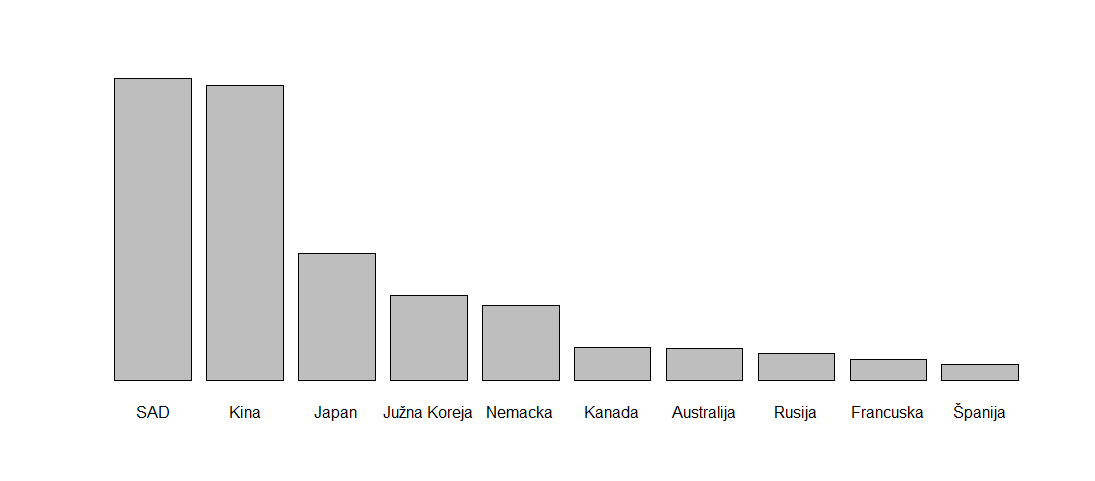
\includegraphics[scale=0.41]{slika.png}
\end{center}
\caption{Broj patenata razvijenih od strane država u oblasti autonomne vožnje}
\label{fig:histograma}
\end{figure} 

\subsection{Pojava etičkih problema}
\label{subsec:Pojava etičkih problema}
Od pomenutih nivoa automatizacije, prva dva uspešno učestvuju u saobraćaju kao pomoć vozačima, dok iako za treći stepen postoje uslovi, ovakva vozila se smatraju samo korakom napred u razvoju autonomnih vozila, iz aspekta nauke, ali nisu od praktičnog značaja iz brojnih etičkih razloga. \\
Naime, takva vožnja zahteva da vozači budu prisutni i da na signal mašine, odnosno vozila, reaguju po potrebi, kako bi rešili neke kritične situacije. Tu se postavljaju pitanja da li je moguce da čovek koji je na trenutke bio okupiran drugim stvarima i nije pažljivo pratio vožnju sve vreme, može dovoljno brzo da reaguje na zahtev mašine i da li će te reakcije biti ispravne? Poznavajući čovekovu prirodu, nije teško zaključiti da je ovakav koncept prilično nepraktičan i da bi samo povećao broj nesreća umesto da ih minimizuje i učini vožnju udobnom i bezbednom što je cilj.

\subsection{Problem tramvaja}
\label{subsec:Pojava etičkih problema}
Jedan od najpoznatijih problema je problem Tramvaja (eng.~{\em Trolley problem}). To je situacija u kojoj se vozilo krece šinama i nailazi na šest osoba koje predstavljaju prepreku na putu, ali jedini način da ih ne udari je da skrene na alternativni put na kome se nalazi jedna osoba, koju, takođe, ne može da zaobiđe.  \\
Poznato je da postoje slučajevi u kojima je nemoguće izbeći nezgodu, pa je neophodno utvrditi mehanizam po kome bi mašine donosile odluke i nekada dovodile do eventualnih žrtava. Pitanje koje se na ovome mestu postavlja je - kako postopiti u ovakvoj situaciji, a da postupak bude etički ispravan? Postojanje odgovora na ovo pitanje bi omogućilo opisivanje ponasanja autonomnog vozila koje bi uvek bilo ispravno u kontekstu etike.

\subsection{Etički okviri}
\label{subsec:Etički okviri}
Težina problema kreiranja autonomnih vozila se krije u preslikavanju ispravnih postupaka u matematičke formule koje se nalaze u osnovi odlučivanja automatskih mašina. U literaturi se najčešće porede sledeća tri okvira:
\begin{itemize}
 \item {Deontološka etika - unapred je definisan skup dobrih i loših postupaka}
 \item {Utilitarizam - svaki postupak maksimizuje korist, pa se u različitim              situacijama isti postupak može pokazati nekada ispravan, a nekada ne }
 \item {Etika rizika - procena i minimizacija rizika}
\end{itemize}
Svaki od ova tri okvira, kao i mnogi drugi koji se spominju u literaturi, imaju svoje mane. Do sada nije zabeleženo rešenje neizbežne nesreće koje zadovoljava sve etičke zahteve. \cite{etika}

\subsubsection{Mane etičkih okvira}
\label{subsubsec:Mane etičkih okvira}
Etika i pravo se ne mogu definisati na jedinstven način - u različitim zemljama se različite stvari smatraju ispravnim, odnosno neispravnim. Mnogo faktora utiče na vozače pri donošenju odluka tokom vožnje, a neke situacije se medju vozačima razrešavaju korišćenjem nekih internih načina sporazumevanja poput pokreta ruke, glave i slično, pa je veoma teško napraviti mašinu koja bi donosila odluke poput ljudi u sličnim situacijama. \\
Sledeće važno pitanje je način donošenja odluka u slučajevima poput Trolley problema. Nešto sa čime se ljudi generalno slažu je da bi čovek, bez obzira na bilo kakve karakteristike, trebalo da ima prednost da preživi u odnosu na životinju. Međutim, teško je doneti odluku kada su jedini učesnici ljudi, kao pešaci ili vozači. Same karakteristike pri \emph{izboru žrtve} ne bi smele da imaju uticaj (pol, rasa, starost ili bilo koja druga fizička karakteristika) jer bi u tom slučaju bilo izuzetno zahtevno postaviti granicu - kada nekoga poštedeti, a kada ne, da li više vredi sačuvati živote nekoliko starijih osoba ili jednoj mlađoj i sl. Međutim, ako se detaljnije razmotri takva situacija, mašina bi uvek birala da poštedi veći broj ljudi, iako bi covek na osnovu svog subjektivnog osećaja nekada mogao da postupi \emph{drugacije}. \\
Još jedan aspekt o kome se može diskutovati je pitanje kako se postupa kada je putnik u autonomnoj mašini ugrožen. On nije osoba koja upravlja vozilom, niti osoba koja je napravila ili programirala isto, pa je svakako bitno težiti ponašanju vozila koje pokušava da zaštiti putnika ukoliko je to moguće. Jedan interesantan primer za diskusiju je situacija u kojoj se sa jedne strane vozila nalazi motor, a sa druge kamion - ukoliko vozilo skrene u pravcu motora, veće su šanse da će vozač motora nastradati, međutim ukoliko vozilo skrene u pravcu kamiona, veće su sanse da putnik tog vozila nastrada. \\
Veoma je teško diskutovati na temu etike kada se ljudi nikada neće usaglasiti oko jedinstvenog etičkog okvira, s toga se može izvesti zaključak da potpuna autonomija vozila nikada neće biti prihvaćena od strane svih pojedinaca.

\subsection{Prednosti autonomne vožnje}
\label{subsec:Prednosti autonomne vožnje}
Pored svih kontraverznih pitanja o kojima je bilo reči, autonomna vožnja ima i brojne prednosti: eliminisanje nesreća usled umora ili stresa vozača, prekoračenja brzine, vožnje pod dejstvom psihoaktivnih supstanci. Takođe ovaj koncept omogućava smanjenje zagađenja zivotne sredine, optimalnu potrošnju i sl.


\end{document}
